\section{Ausblick auf zukünftige Ergänzungen} \label{sec:praktischeUmsetzung:ausblick}

\subsection{Zugriff auf Personendaten und Auswertungen}
Die Auswertung der erbrachten Leistungen einzelner Personen ist aus regulatorischen Gründen ein komplexes Thema und erfordert die Zustimmung des Betriebsrates. Für die meisten Benutzer könnte dies über eine Gruppe mit entsprechenden Rechten im \ac{aad} gelöst werden, in der die Mitglieder vom Betriebsrat verwaltet werden. Datenbankadministratoren hätten jedoch immer noch die Möglichkeit, auf die Personendaten zuzugreifen. 

Mit der Datenbankfunktion \textit{Always Encrypted} kann das verhindert werden. \textit{Always Encrypted} ermöglicht es Spalten zu verschlüsseln und kann damit auch Datenbankadministratoren daran hindern sensitive Daten zu lesen. Der verwendete Schlüssel wird im \textit{Key Vault} gespeichert und die dort eingestellten Zugriffsberechtigungen auf den Schlüssel, bestimmen, wer die Daten unverschlüsselt abfragen kann. Die Entschlüsselung während der Abfrage passiert dabei automatisch \cite{mauri_practical_2021}. Es wäre demnach ausreichend, der zuvor erstellten Gruppe, Zugriff auf den Schlüssel im \textit{Key Vault} zu gewähren. Einem Datenbankadministrator, der nicht in dieser Gruppe ist, werden dann nur verschlüsselte Binärwerte angezeigt. 

\subsection{Einbindung von Azure Machine Learning für fortgeschrittene Analysen} \label{sec:praktischeUmsetzung:ausblick:aml}

\begin{figure}[htbp]
 \centering
 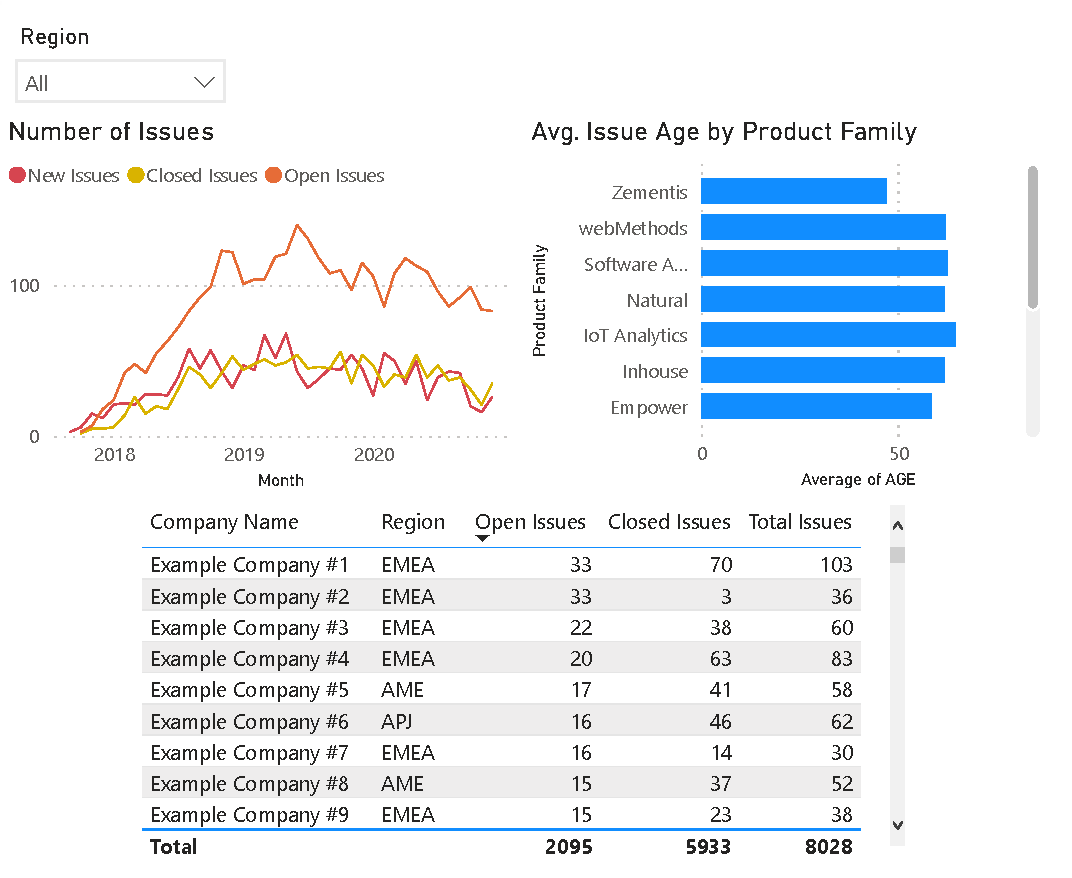
\includegraphics[width=\textwidth]{gfx/pbi_report.pdf}
 \caption[Azure Machine Learning]{Ergänzung von Azure Machie Learning (unvollständig)}
\label{fig:praktischeUmsetzung:ausblick:aml}
\end{figure}